\documentclass{article}
\usepackage{geometry}
\geometry{a4paper, margin=1in}
\usepackage{graphicx}
\usepackage[hidelinks]{hyperref}
\usepackage{amsmath}
\usepackage{float}
\usepackage{bookmark}
\usepackage[inline,shortlabels]{enumitem}
\begin{document}

% Cover Page
\begin{titlepage}
	\centering
	\vspace*{1cm}

	
\includegraphics[width=0.5\textwidth]{assets/logo.png}\par\vspace{1cm}

	\Huge
	\textbf{Estimation of Change in Population of Municipalities in PR}

	\vspace{0.5cm}
	\LARGE
	[ESMA 6835]: Bayesian Inference

	\vspace{1.5cm}

	\textbf{Alejandro M. Ouslan \& Tatiana E. Crespo}

	\vfill

	\Large

	\vspace{0.8cm}

	\Large
	University of Puerto Rico, Mayagüez \\
	{\small \today}

\end{titlepage}

\newpage


\tableofcontents

\newpage

%------------------------------------------------
\section{Introduction}
%------------------------------------------------

Changes in demographics are a highly studied topic and are of great interest to governments. Understanding demographic characteristics is particularly important for regional governments, such as the municipalities in Puerto Rico. Anticipating how the population will change in the coming years is fundamental for planning infrastructure projects and public investments, especially in areas experiencing population growth, decline, or aging populations.

Classical inference methods, such as classical linear regression, are frequently used to study these trends. However, applying Bayesian inference methods offers significant advantages. This is due to the ability to incorporate prior information and provide complete probability distributions for the estimated parameters.

Based on these arguments, we are led to ask the following questions: How has the population of a municipality in Puerto Rico changed over time? Therefore, through this project, we will use simple linear regression with a Bayesian approach to estimate and analyze population change in Puerto Rican municipalities over time.



%------------------------------------------------
\section{Methodology}
%------------------------------------------------
\subsection{Data}
This research uses data from the American Community Survey 5-year estimates (ACS)
produced by the U.S. Census Bureau. The dataset includes population estimates from
2011 to 2023 for all 78 municipalities in Puerto Rico.

The variables to consider for our simple regression model are: the years for which we have population estimates for Puerto Rico (independent variable X) and the total population for the 78 municipalities of Puerto Rico for each year (dependent variable Y).

\subsection{Regression Model}

The simple linear regression model to be used is the following:

\[
	Y_i = \beta_0 + \beta_1 X_i + \epsilon_i
\]

where:
\begin{itemize}
	\item $Y_i = $ population in year $i$
	\item $X_i = $ year
	\item $\beta_0 = $ intercept
	\item $\beta_1 = $ population change rate
	\item $\epsilon_i = $ random error
\end{itemize}

\subsection{Bayesian Approach}

Due to the nature of the Bayesian approach, we will use non-informative prior distributions. However, we will use the Markov Chain Monte Carlo method to obtain the posterior distributions of the data. This process will be executed in Python software.


%------------------------------------------------
\section{Results}
%------------------------------------------------

A classical linear regression was performed with a significance level of $\alpha = 0.05$, from which we obtained a population change rate of $-210.52$, indicating that the total population decreases each year. However, upon reviewing the p-value of this test (0.540), we realized that our findings are not statistically significant. Therefore, based on classical inference, there is insufficient evidence to determine that there is a drastic change in the population decrease over time in this model. Moreover, since the adjusted R-squared is $-0.001$ this indicates that the model with the variable time might not be the best to explain the changes in populations.

Regarding the Bayesian regression, we obtained that the mean of the posterior distribution of the coefficient corresponding to the years is $-211.04$. This indicates that the population decreases per year. Furthermore, reviewing the Bayesian confidence intervals, it was found that there is a 94\% probability that the year effect is between -822.54 and 444.45. According to the credibility intervals, with 94\% confidence, the expected coefficient for years is between -500.00 and 50.00. Because this interval includes zero, there is no statistically significative probability that the effect of years is negative. Regarding the MCMC chains, the chains appear to blend quite well, and the R-squared value is approximately 1, suggesting that the model converged correctly. Although both classical and Bayesian inference essentially conclude that the population rate of change and the model do not answer our question, the Bayesian inference method is more robust. This is due to the fact that the Bayesian method uses prior information to perform the analyses. This allows the model to be normalized, reduces model identification problems, and makes the estimators less unstable.


%------------------------------------------------
\section{Predicciones}
%------------------------------------------------

Due to the lack of statistical significance in the results regarding changes over time in municipal population, no meaningful recommendations can be made regarding the problem.



%------------------------------------------------
\section{Conclusions}
%------------------------------------------------

The overall results of the simple regression are inconclusive, as the variable representing
year was not statistically significant. This lack of statistical significance may be due to
the limitations of simple regression models. A major limitation is the violation of the
assumption of independence and identical distribution (i.i.d.), since population values are
highly correlated with those of the previous year. It is advisable to use a more appropriate
model for time series data, such as an ARIMA model.


\section*{Appendix A: Simple regression}

\begin{table}[ht]
	\centering
	\caption{OLS Regression Results}
	\begin{tabular}{lcccccc}
		\hline
		\textbf{Variable}    & \textbf{Coefficient} & \textbf{Std. Error} & \textbf{t-Statistic} & \textbf{P-value} & \textbf{95\% CI}    \\
		\hline
		Intercept            & 461,000              & 693,000             & 0.666                & 0.506            & [-899,000, 1.82M]   \\
		Year                 & -210.515             & 343.336             & -0.613               & 0.540            & [-884.247, 463.216] \\
		\hline
		\textbf{Model Fit}   &                      &                     &                      &                  &                     \\
		\hline
		R-squared            & 0.000                &                     &                      &                  &                     \\
		Adjusted R-squared   & -0.001               &                     &                      &                  &                     \\
		F-statistic          & 0.3759               &                     &                      & 0.540            &                     \\
		Prob (F-statistic)   &                      &                     &                      & 0.540            &                     \\
		No. Observations     & 1014                 &                     &                      &                  &                     \\
		\hline
		\textbf{Diagnostics} &                      &                     &                      &                  &                     \\
		\hline
		Omnibus              & 898.513              &                     &                      & 0.000            &                     \\
		Jarque-Bera          & 22,245.704           &                     &                      & 0.000            &                     \\
		Skew                 & 4.144                &                     &                      &                  &                     \\
		Kurtosis             & 24.397               &                     &                      &                  &                     \\
		Durbin-Watson        & 1.935                &                     &                      &                  &                     \\
		Condition No.        & 1.09e+06             &                     &                      &                  &                     \\
		\hline
	\end{tabular}
\end{table}

\begin{table}[ht]
	\centering
	\caption{Bayes simple regression Results (Mean, SD, HDI)}
	\begin{tabular}{lcccccc}
		\hline
		\textbf{Variable} & \textbf{Mean} & \textbf{SD} & \textbf{HDI 3\%} & \textbf{HDI 97\%} \\
		\hline
		Intercept         & 479,133.653   & 704,469.055 & -922,695.260     & 1,743,484.519     \\
		Sigma             & 40,914.524    & 917.309     & 39,261.811       & 42,711.419        \\
		Year              & -219.481      & 349.280     & -847.946         & 473.013           \\
		\hline
	\end{tabular}
\end{table}

\begin{table}[ht]
	\centering
	\caption{Bayes simple regression Results (MCSE, ESS, and R-hat)}
	\begin{tabular}{lccccccccc}
		\hline
		\textbf{Variable} & \textbf{MCSE Mean} & \textbf{MCSE SD} & \textbf{ESS Bulk} & \textbf{ESS Tail} & \textbf{R-hat} \\
		\hline
		Intercept         & 9,270.616          & 11,465.597       & 5,768.0           & 2,821.0           & 1.0            \\
		Sigma             & 11.705             & 14.697           & 6,165.0           & 3,085.0           & 1.0            \\
		Year              & 4.597              & 5.685            & 5,767.0           & 2,821.0           & 1.0            \\
		\hline
	\end{tabular}
\end{table}


\begin{figure}[H]
	\centering
	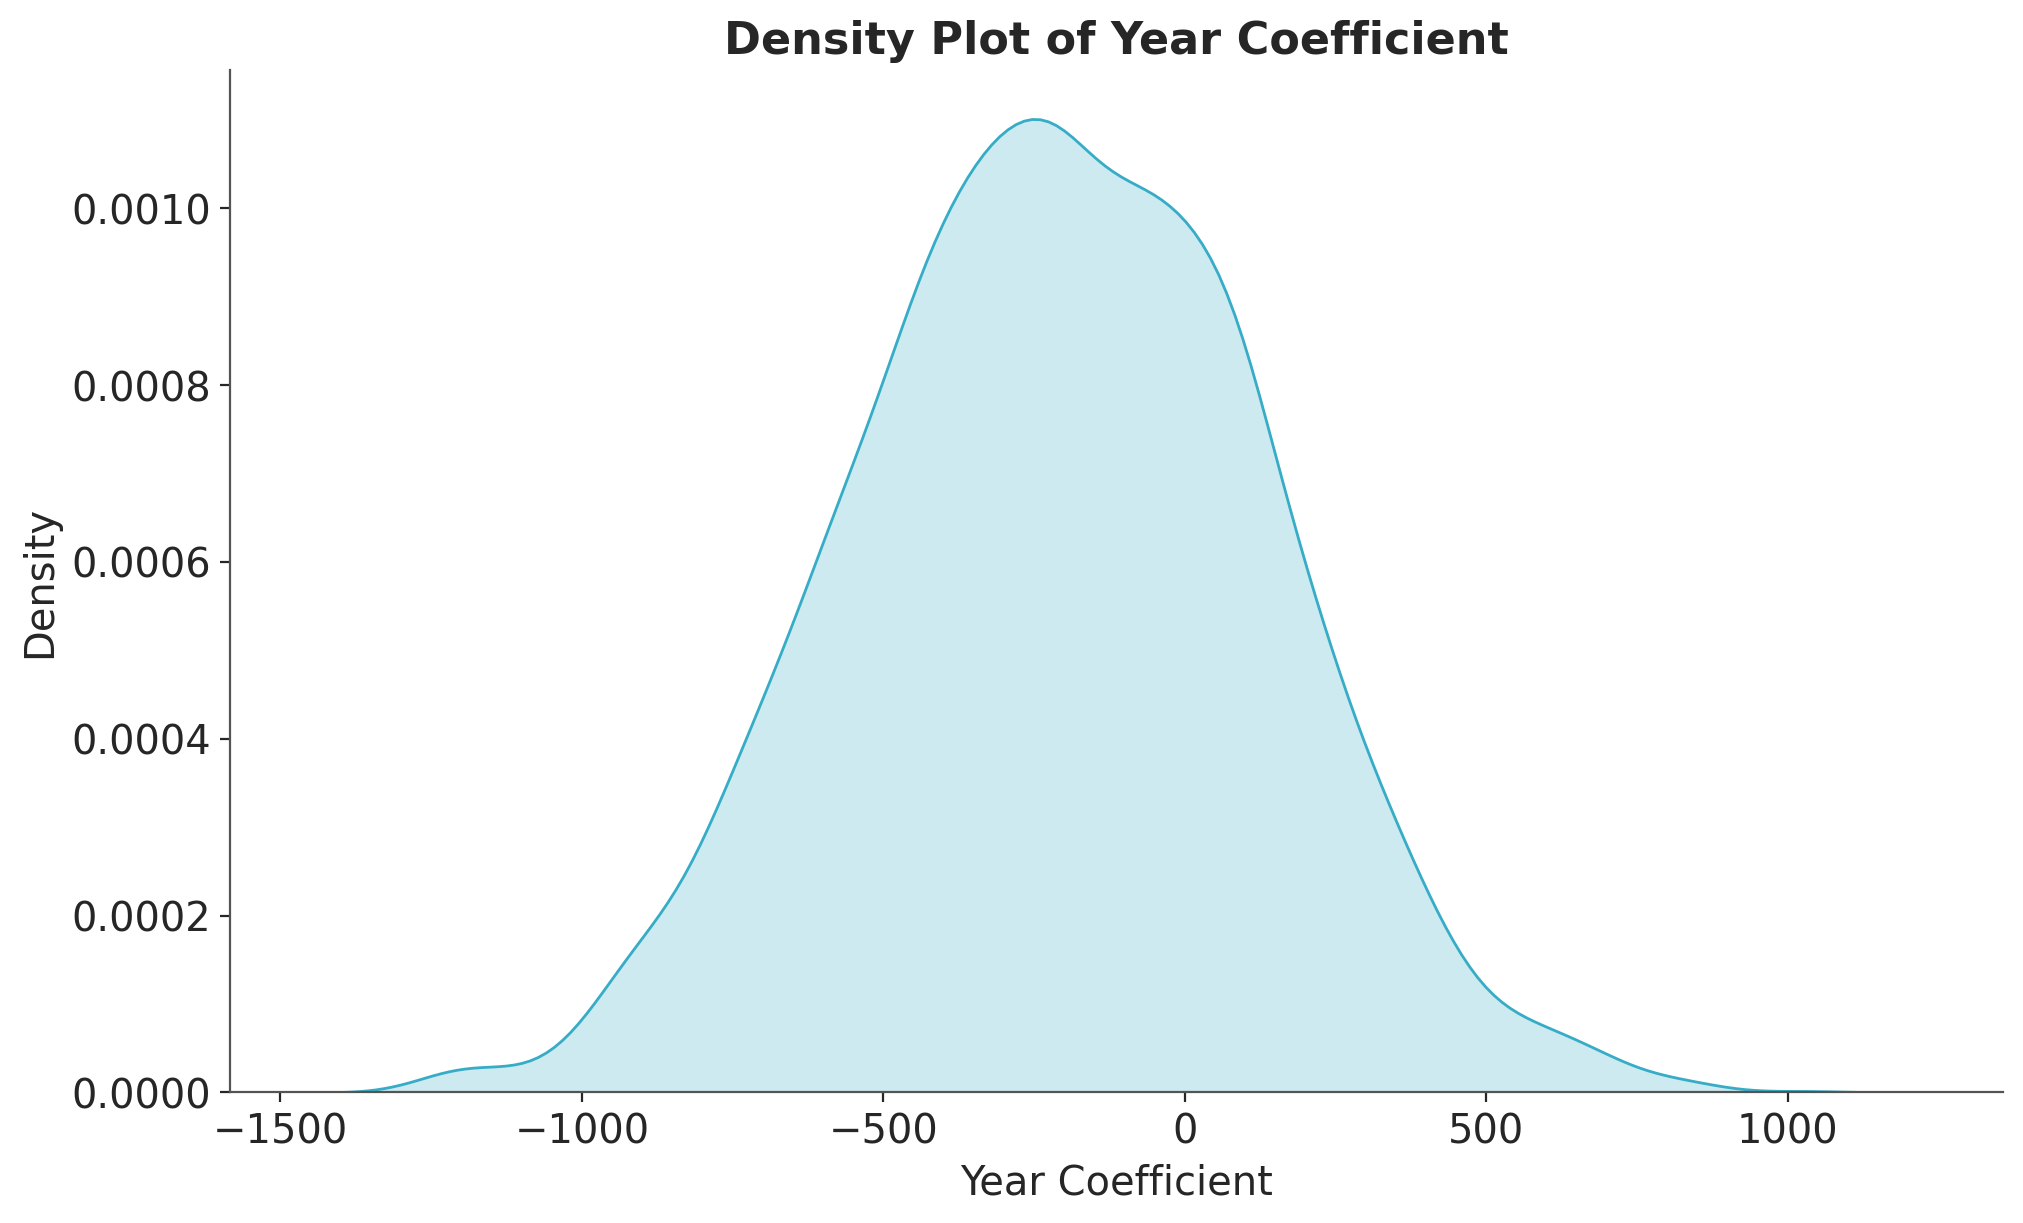
\includegraphics[width=0.4\textwidth]{assets/density.png}
	\caption{Density of simple regression}
\end{figure}

\begin{figure}[H]
	\centering
	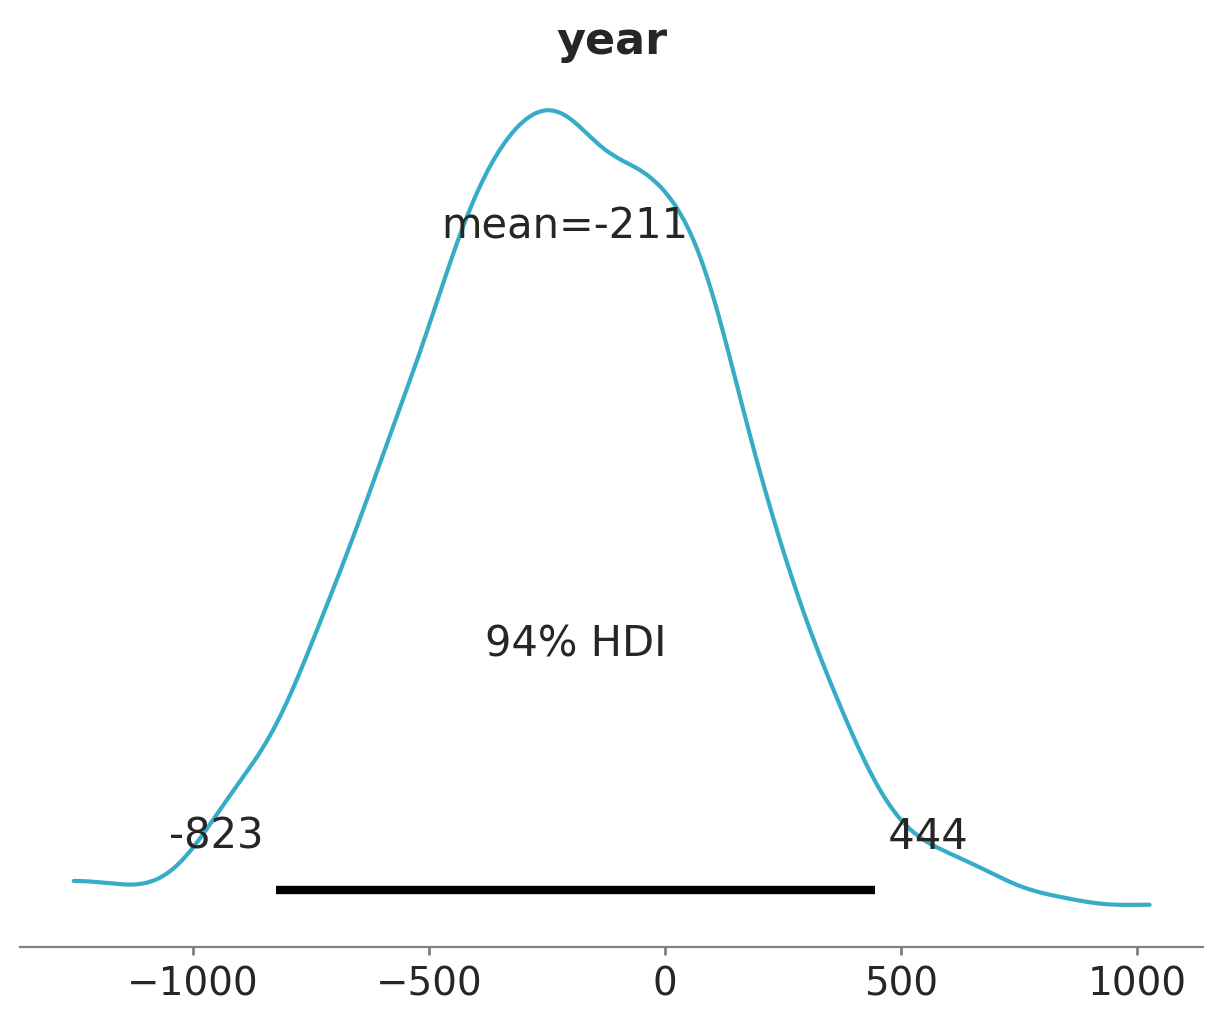
\includegraphics[width=0.4\textwidth]{assets/confidence.png}
	\caption{Confidence interval of Simple regression}
\end{figure}

\begin{figure}[H]
	\centering
	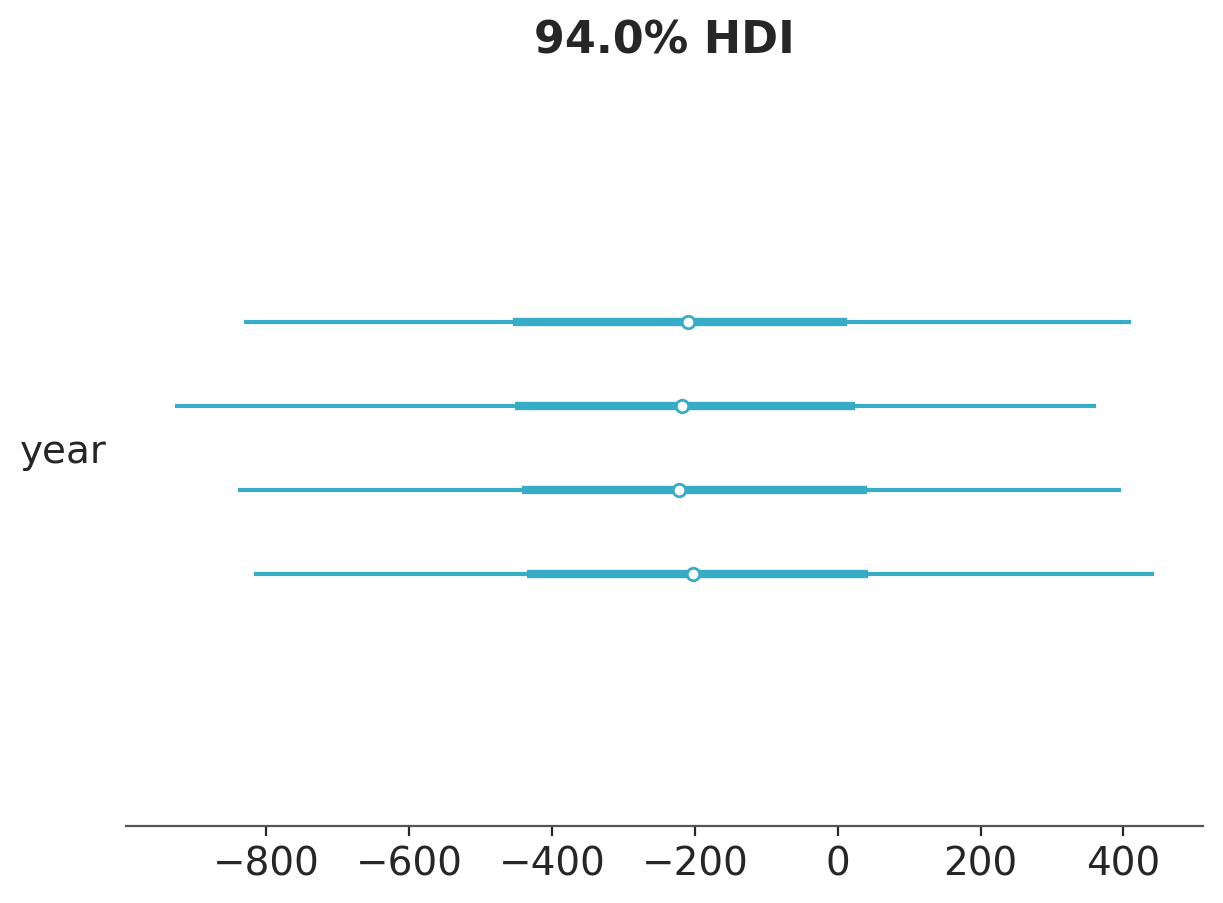
\includegraphics[width=0.4\textwidth]{assets/credibility intervals.png}
	\caption{Credibility interval of Simple regression}
\end{figure}

\begin{figure}[H]
	\centering
	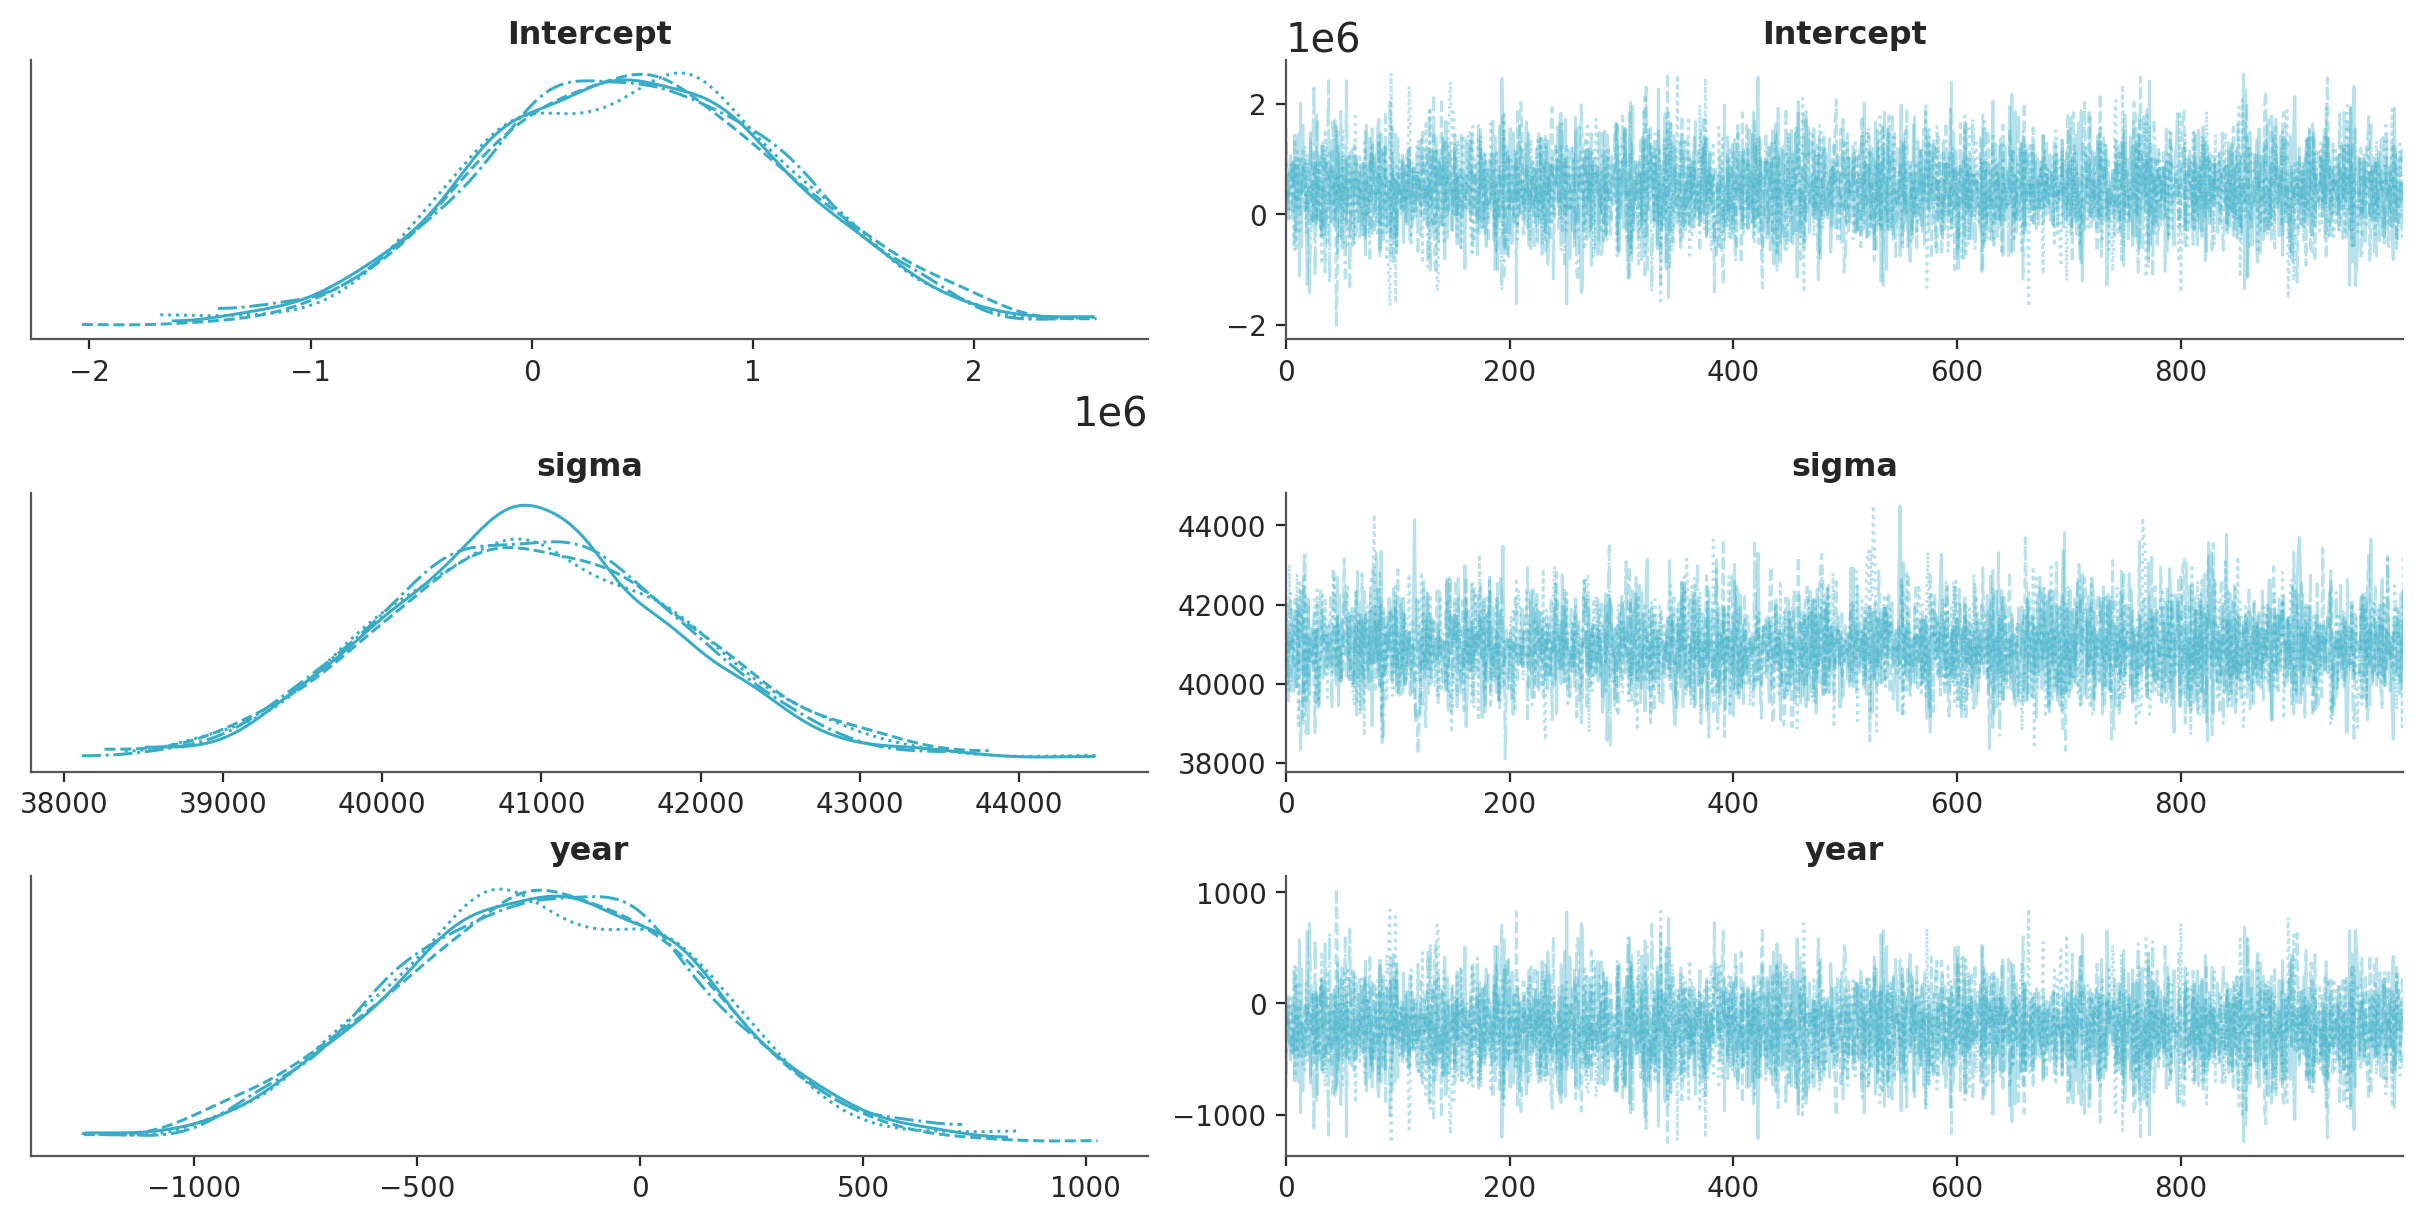
\includegraphics[width=0.4\textwidth]{assets/trace.png}
	\caption{Trace graph of simple regression}
\end{figure}


\section*{Appendix B: Log regression}

\begin{table}[ht]
	\centering
	\caption{OLS Regression Results (Model Fit and Coefficients)}
	\begin{tabular}{lcccccc}
		\hline
		\textbf{Variable}  & \textbf{Coef} & \textbf{Std. Error} & \textbf{t-Statistic} & \textbf{P-value} & \textbf{95\% CI} \\
		\hline
		Intercept          & 20.8794       & 13.317              & 1.568                & 0.117            & [-5.254, 47.012] \\
		Year               & -0.0053       & 0.007               & -0.804               & 0.422            & [-0.018, 0.008]  \\
		\hline
		\textbf{Model Fit} &               &                     &                      &                  &                  \\
		\hline
		R-squared          & 0.001         &                     &                      &                  &                  \\
		Adjusted R-squared & -0.000        &                     &                      &                  &                  \\
		F-statistic        & 0.6461        &                     &                      & 0.422            &                  \\
		Prob (F-statistic) &               &                     &                      & 0.422            &                  \\
		No. Observations   & 1014          &                     &                      &                  &                  \\
		\hline
	\end{tabular}
\end{table}

\begin{table}[ht]
	\centering
	\caption{Bayesian Sampling Results (Mean, SD, HDI)}
	\begin{tabular}{lcccccc}
		\hline
		\textbf{Variable} & \textbf{Mean} & \textbf{SD} & \textbf{HDI 3\%} & \textbf{HDI 97\%} \\
		\hline
		Intercept         & 20.846        & 13.403      & -4.771           & 46.100            \\
		Sigma             & 0.788         & 0.018       & 0.756            & 0.822             \\
		Year              & -0.005        & 0.007       & -0.018           & 0.007             \\
		\hline
	\end{tabular}
\end{table}


\begin{table}[ht]
	\centering
	\caption{Bayesian Sampling Results (MCSE, ESS, and R-hat)}
	\begin{tabular}{lcccccccc}
		\hline
		\textbf{Variable} & \textbf{MCSE Mean} & \textbf{MCSE SD} & \textbf{ESS Bulk} & \textbf{ESS Tail} & \textbf{R-hat} \\
		\hline
		Intercept         & 0.17               & 0.226            & 6221.0            & 2891.0            & 1.0            \\
		Sigma             & 0.00               & 0.000            & 6424.0            & 2900.0            & 1.0            \\
		Year              & 0.00               & 0.000            & 6217.0            & 2865.0            & 1.0            \\
		\hline
	\end{tabular}
\end{table}

\begin{figure}[H]
	\centering
	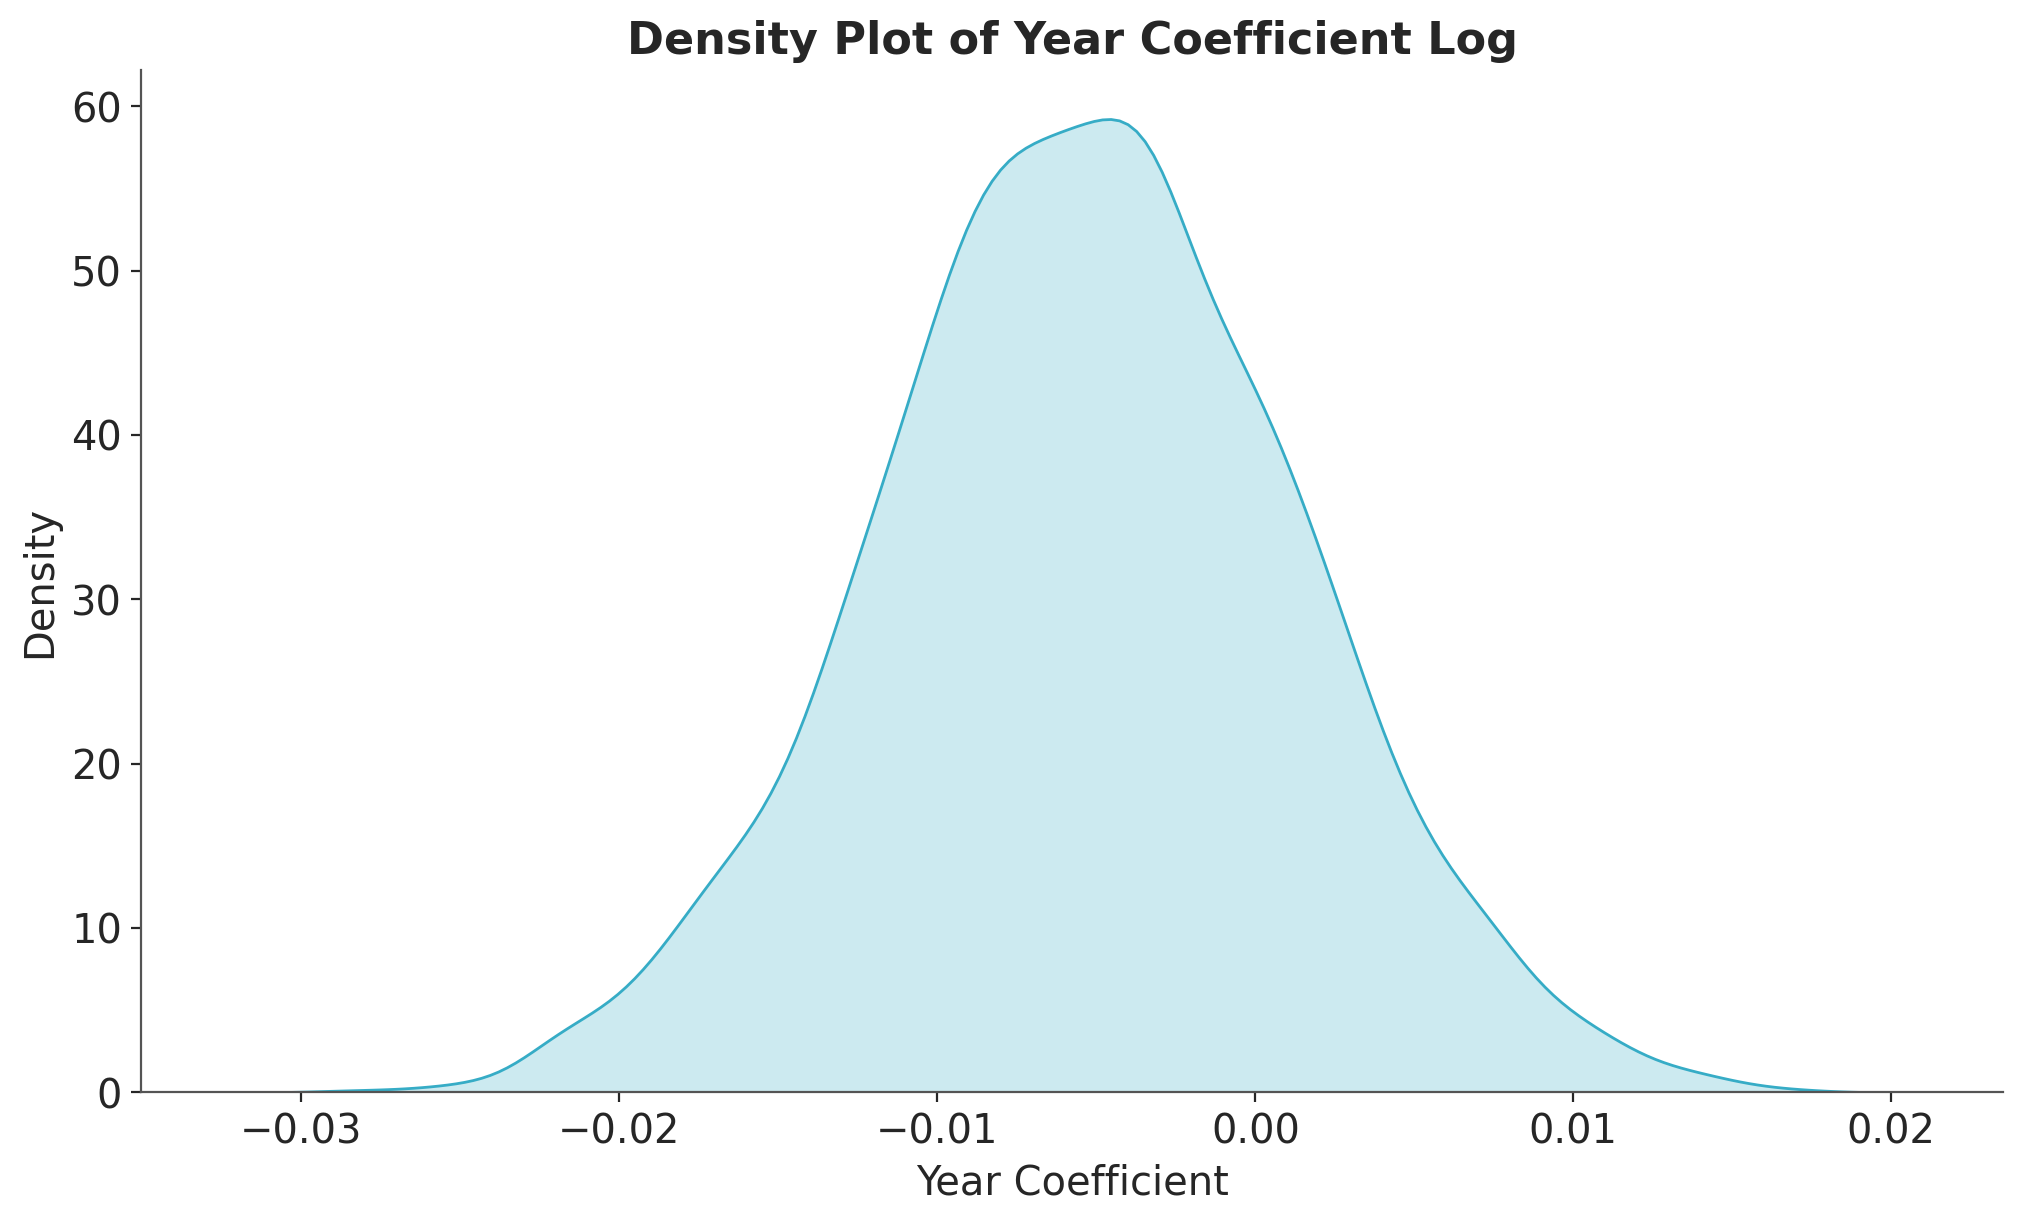
\includegraphics[width=0.4\textwidth]{assets/log_density.png}
	\caption{Density of Log regression}
\end{figure}

\begin{figure}[H]
	\centering
	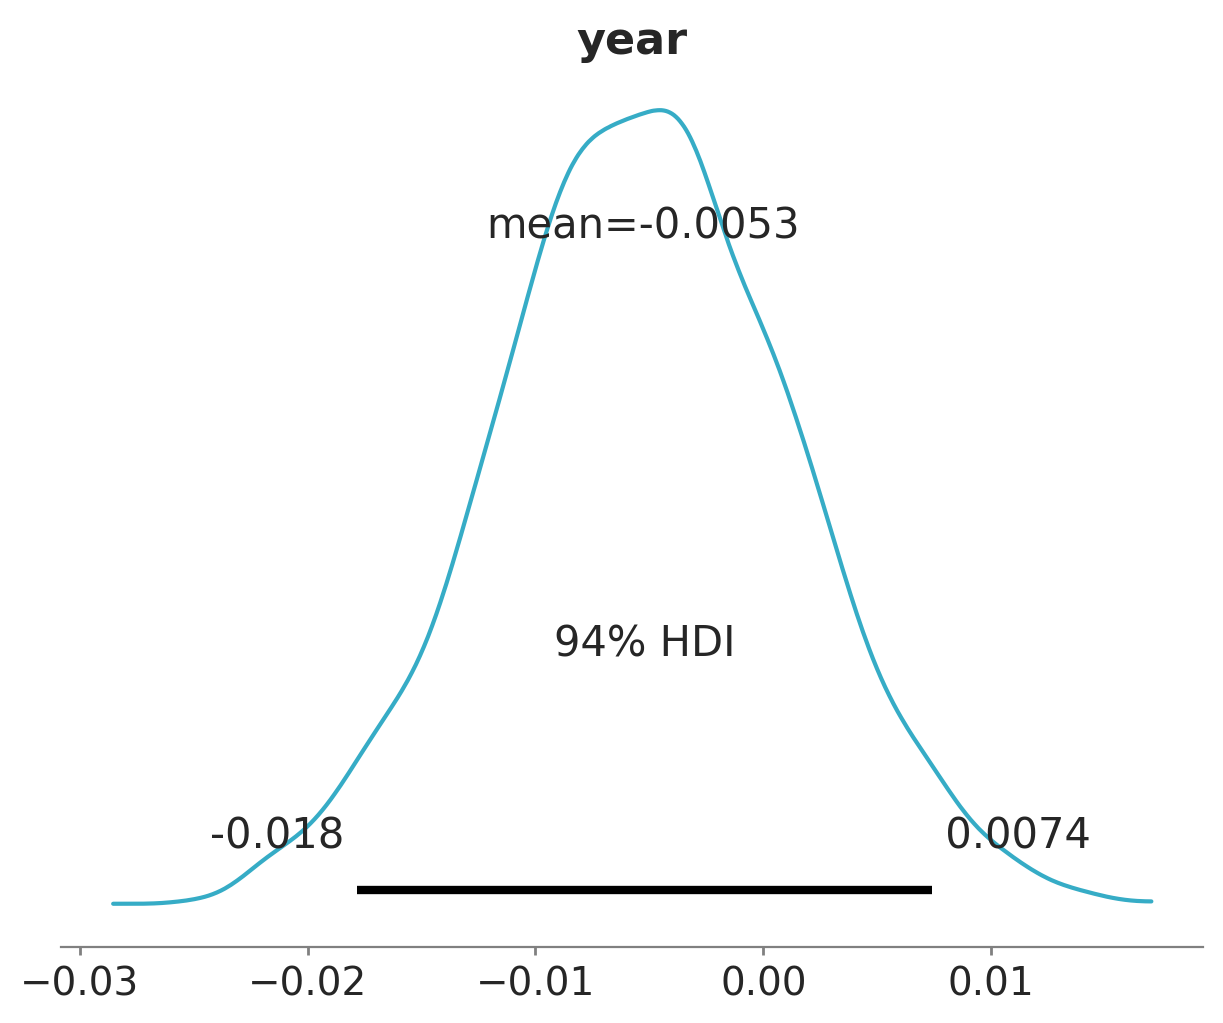
\includegraphics[width=0.4\textwidth]{assets/log_confidence.png}
	\caption{Confidence interval of Log regression}
\end{figure}

\begin{figure}[H]
	\centering
	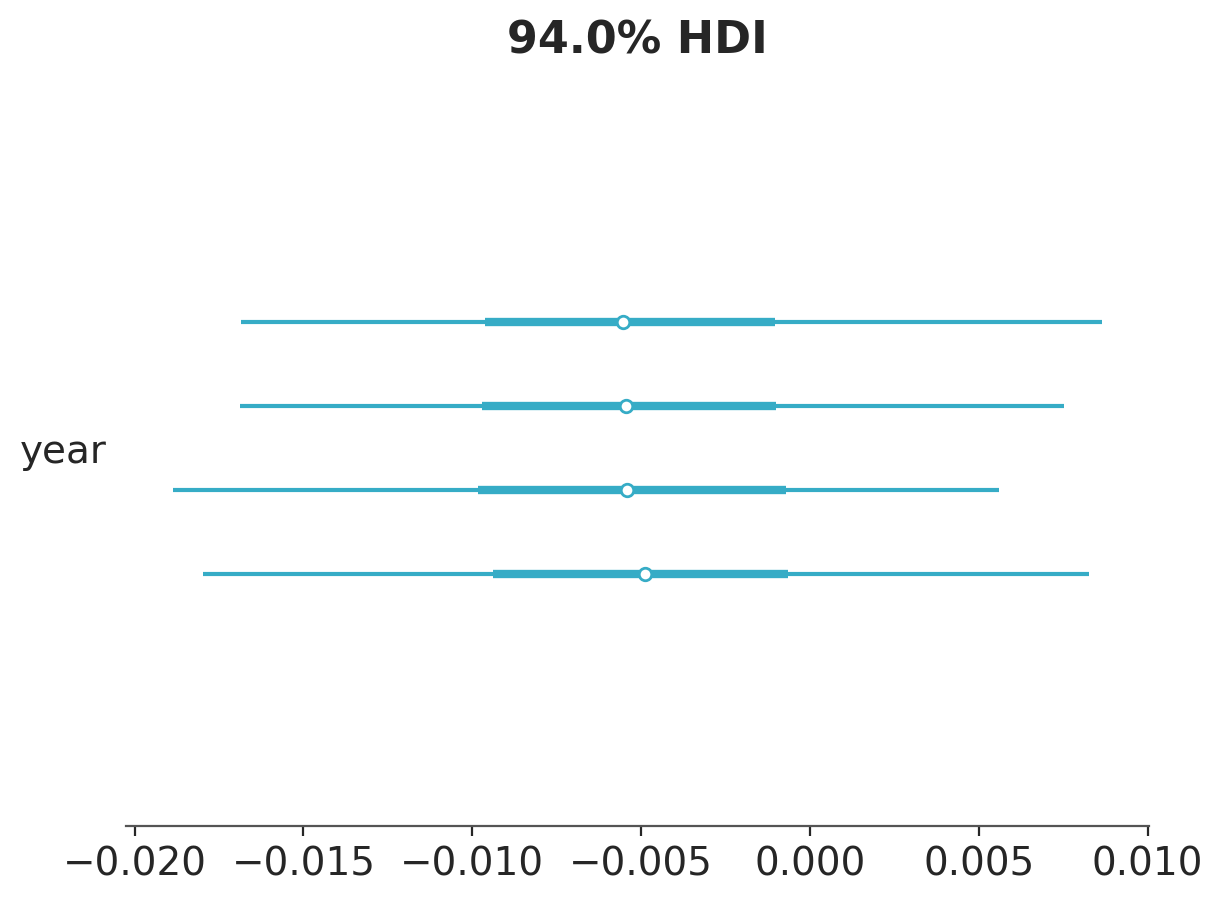
\includegraphics[width=0.4\textwidth]{assets/log_credibility.png}
	\caption{Credibility interval of Log regression}
\end{figure}

\section{Appendix C: Log fixed effect}

\begin{table}[ht]
	\centering
	\caption{OLS Regression Results (Model Fit and Initial Coefficients)}
	\begin{tabular}{lcccccc}
		\hline
		\textbf{Variable}    & \textbf{Coef} & \textbf{Std. Error} & \textbf{t-Statistic} & \textbf{P-value} & \textbf{95\% CI} \\
		\hline
		Intercept            & 20.3180       & 0.517               & 39.291               & 0.000            & [19.303, 21.333] \\
		C(county)[T.3.0]     & 0.7826        & 0.012               & 65.330               & 0.000            & [0.759, 0.806]   \\
		C(county)[T.5.0]     & 1.1297        & 0.012               & 94.300               & 0.000            & [1.106, 1.153]   \\
		C(county)[T.7.0]     & 0.3701        & 0.012               & 30.898               & 0.000            & [0.347, 0.394]   \\
		C(county)[T.9.0]     & 0.2939        & 0.012               & 24.537               & 0.000            & [0.270, 0.317]   \\
		C(county)[T.11.0]    & 0.4228        & 0.012               & 35.290               & 0.000            & [0.399, 0.446]   \\
		\hline
		\textbf{Model Fit}   &               &                     &                      &                  &                  \\
		\hline
		R-squared            & 0.999         &                     &                      &                  &                  \\
		\textbf{Diagnostics} &               &                     &                      &                  &                  \\
		\hline
		AIC                  & -4122         &                     &                      &                  &                  \\
		BIC                  & -3733         &                     &                      &                  &                  \\
		Df Residuals         & 935           &                     &                      &                  &                  \\
		Df Model             & 78            &                     &                      &                  &                  \\
		Condition No.        & 1.09e+06      &                     &                      &                  &                  \\
		\hline
	\end{tabular}
\end{table}



\begin{table}[ht]
	\centering
	\caption{Bayesian Fixed Effect Results (Mean, SD, HDI)}
	\begin{tabular}{lcccccc}
		\hline
		\textbf{Variable} & \textbf{Mean} & \textbf{SD} & \textbf{HDI 3\%} & \textbf{HDI 97\%} \\
		\hline
		Intercept         & 20.444        & 13.228      & -3.724           & 45.340            \\
		C(county)         & 0.000         & 0.001       & -0.001           & 0.001             \\
		Sigma             & 0.788         & 0.017       & 0.755            & 0.821             \\
		Year              & -0.005        & 0.007       & -0.017           & 0.007             \\
		\hline
	\end{tabular}
\end{table}


\begin{table}[ht]
	\centering
	\caption{Bayesian Fixed Effect Results (MCSE, ESS, and R-hat)}
	\begin{tabular}{lcccccccc}
		\hline
		\textbf{Variable} & \textbf{MCSE Mean} & \textbf{MCSE SD} & \textbf{ESS Bulk} & \textbf{ESS Tail} & \textbf{R-hat} \\
		\hline
		Intercept         & 0.155              & 0.201            & 7236.0            & 3122.0            & 1.0            \\
		C(county)         & 0.000              & 0.000            & 6710.0            & 3373.0            & 1.0            \\
		Sigma             & 0.000              & 0.000            & 7065.0            & 3154.0            & 1.0            \\
		Year              & 0.000              & 0.000            & 7238.0            & 3049.0            & 1.0            \\
		\hline
	\end{tabular}
\end{table}


\begin{table}[ht]
	\centering
	\caption{Bayesian Sampling Results (MCSE, ESS, and R-hat)}
	\begin{tabular}{lcccccccc}
		\hline
		\textbf{Variable} & \textbf{MCSE Mean} & \textbf{MCSE SD} & \textbf{ESS Bulk} & \textbf{ESS Tail} & \textbf{R-hat} \\
		\hline
		Intercept         & 0.17               & 0.226            & 6221.0            & 2891.0            & 1.0            \\
		Sigma             & 0.00               & 0.000            & 6424.0            & 2900.0            & 1.0            \\
		Year              & 0.00               & 0.000            & 6217.0            & 2865.0            & 1.0            \\
		\hline
	\end{tabular}
\end{table}

\begin{figure}[H]
	\centering
	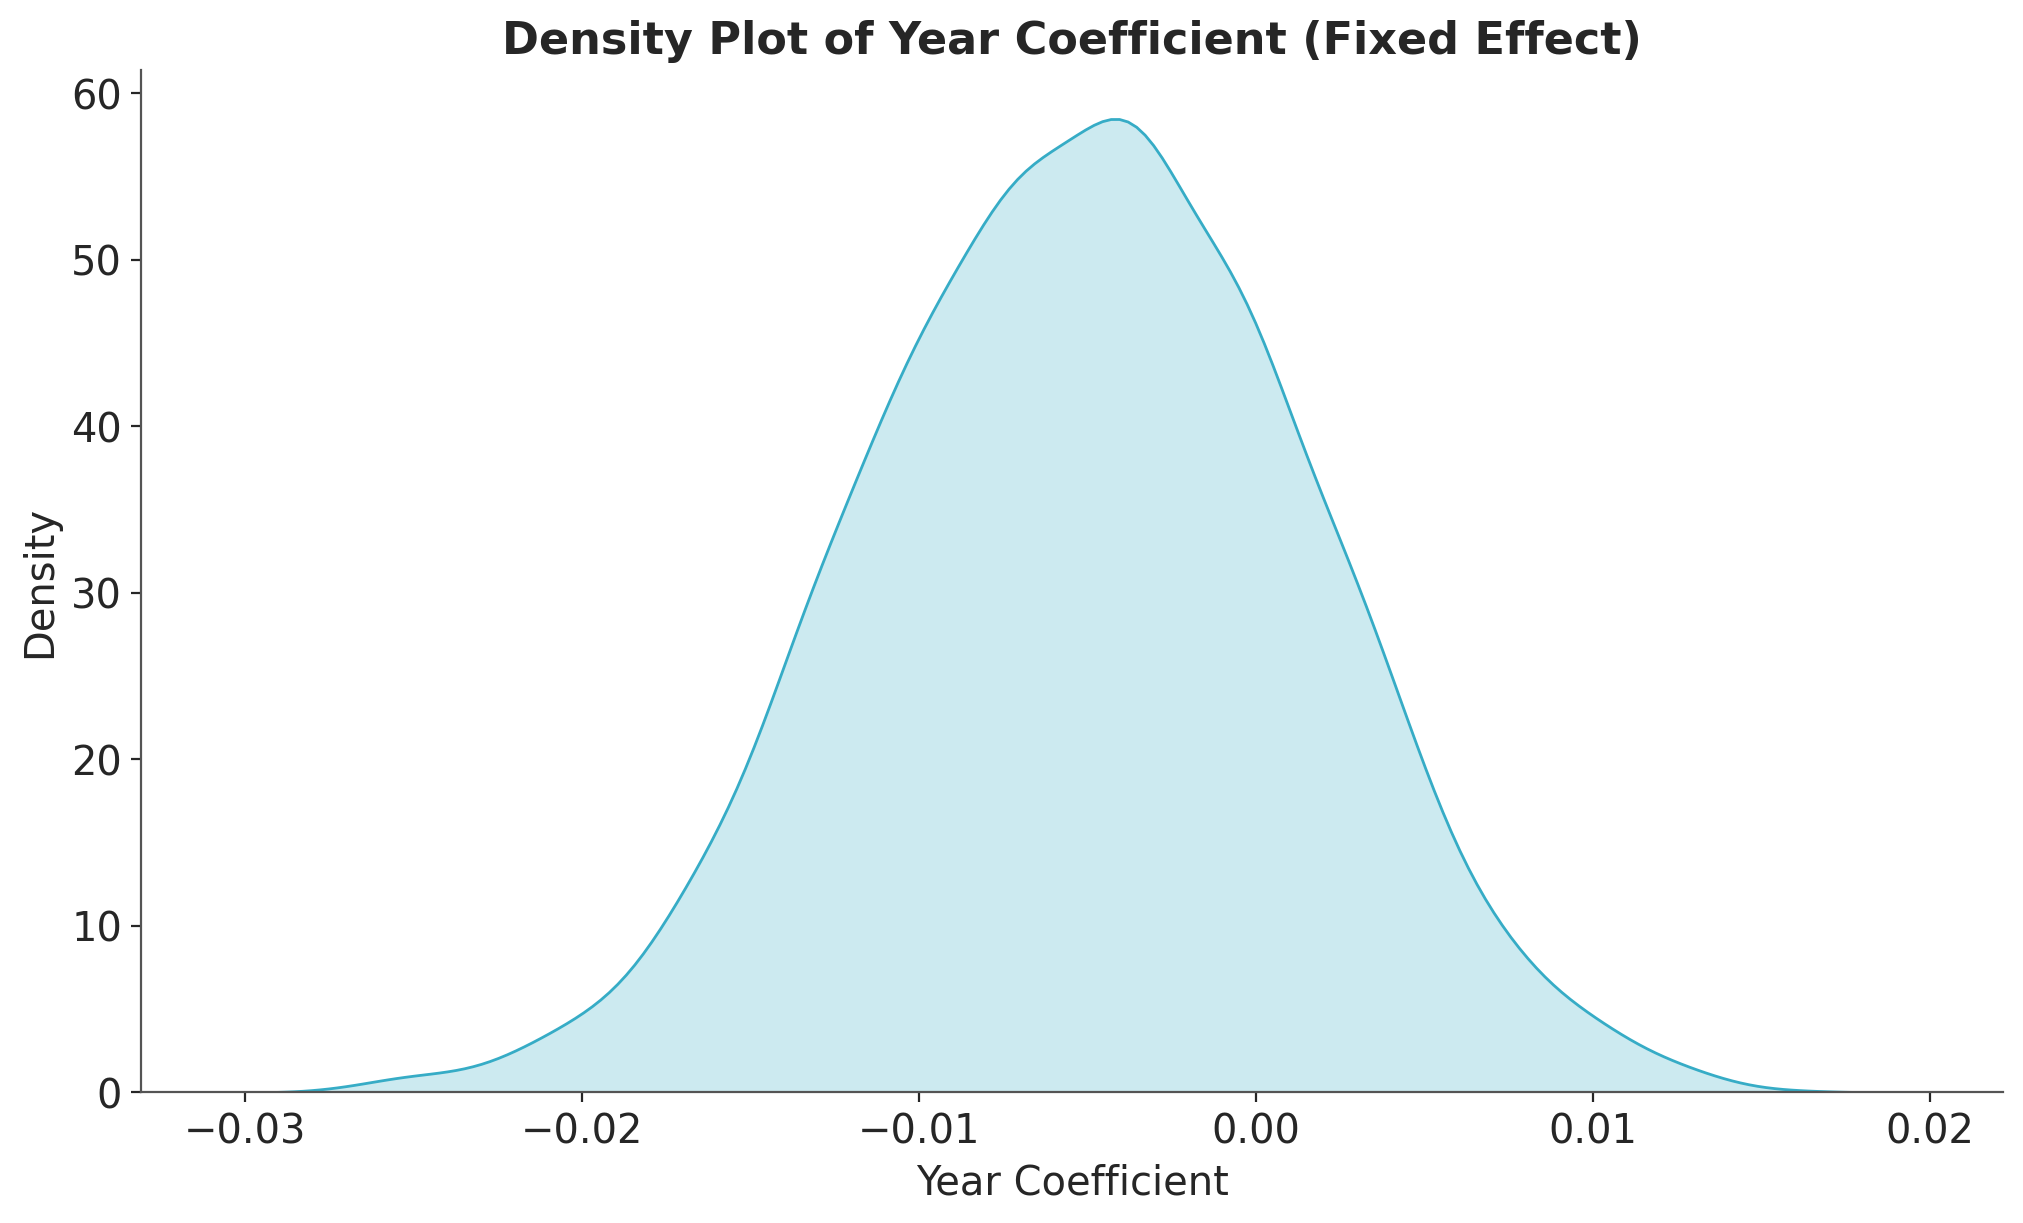
\includegraphics[width=0.4\textwidth]{assets/fix_density.png}
	\caption{Density of fix effect regression}
\end{figure}

\begin{figure}[H]
	\centering
	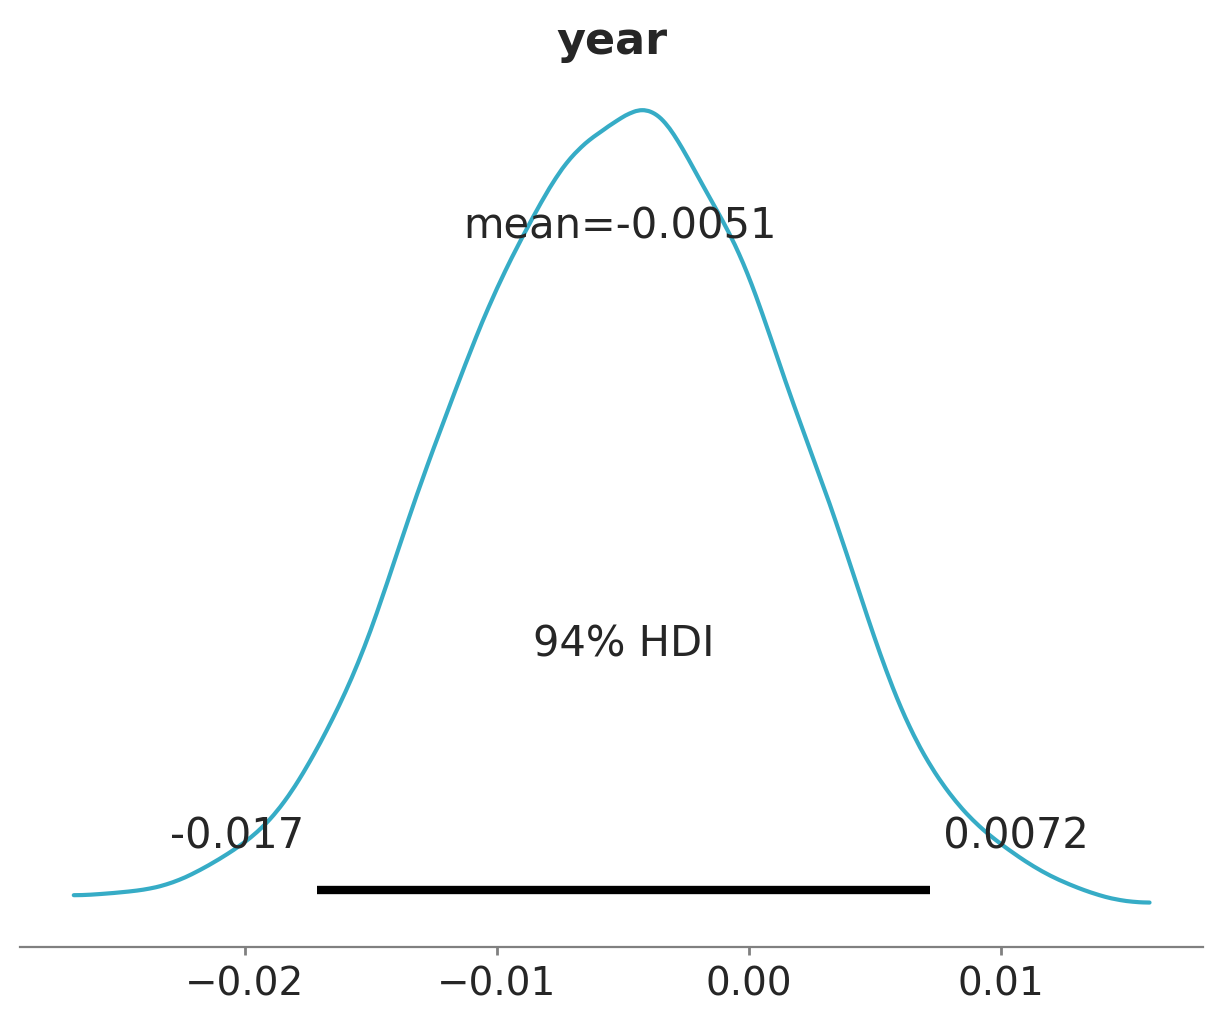
\includegraphics[width=0.4\textwidth]{assets/fix_confidence.png}
	\caption{Confidence interval of fix effect regression}
\end{figure}

\begin{figure}[H]
	\centering
	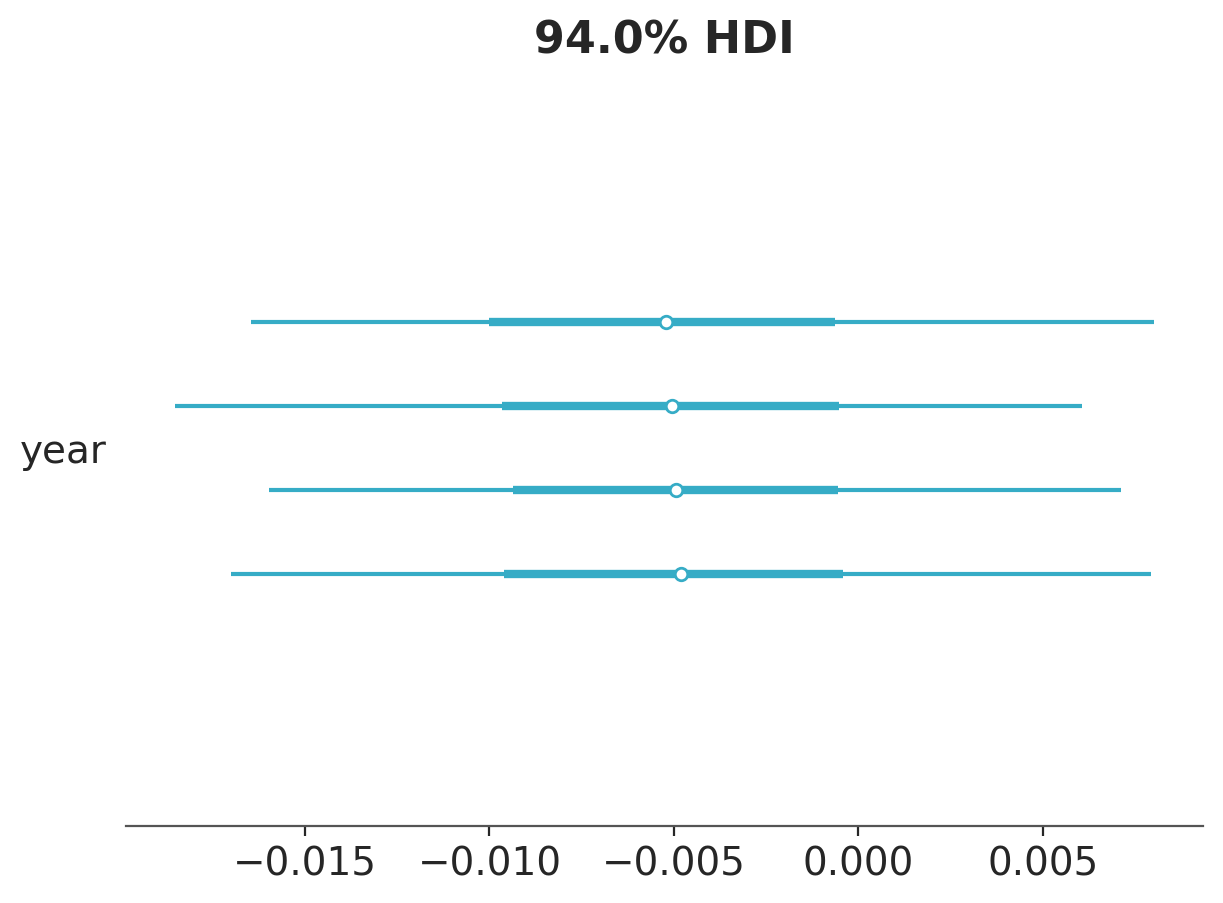
\includegraphics[width=0.4\textwidth]{assets/fix_credibility.png}
	\caption{Credibility interval of Fix effect regression}
\end{figure}


\end{document}
